\documentclass[12pt,a4paper]{article} % Defines the document as an article with 12pt font on A4 paper
\usepackage[utf8]{inputenc} % Sets UTF-8 encoding
\usepackage{geometry} % Enables page geometry customization
\geometry{margin=1in} % Sets 1-inch margins
\usepackage{graphicx} % Allows inclusion of images
\usepackage{titlesec} % Controls section formatting
\usepackage{hyperref} % Enables hyperlinks
\usepackage{tikz}
\usetikzlibrary{shapes.geometric, calc}
\usepackage{setspace} % Allows line spacing adjustments
\usepackage{csquotes} % Improves quotation handling
\usepackage{datetime} % Provides date and time formatting
\usepackage[backend=biber,style=apa, sorting=nyt]{biblatex} % Configures bibliography using Biber with APA style
\addbibresource{references.bib} % Adds a bibliography file (replace with your .bib file name)
\renewcommand{\dateseparator}{-} % Sets date separator as '-'
\onehalfspacing % Sets line spacing to 1.5


\title{\textbf{Research Proposal: PhD candidate in Industrial Engineering}} % Defines the title
\author{
	\textbf{Benjamin R. Berton}\\
	Polytechnique Montréal\\
	\href{mailto:benjamin.berton@polymtl.ca}{benjamin.berton@polymtl.ca}\\
	\textit{Supervised by: Philippe Doyon-Poulin}
} % Defines author details

\begin{document} % Begins the document
	\maketitle % Generates the title
	
	\begin{center}
		\textbf{A cognitive modelling approach to evaluating Human-Autonomy Teaming in commercial aviation}
	\end{center} % Centers the research title
	
	\begin{center}
		Submitted to members of the Jury:\\
		Pr. Jean-Marc Frayret, Pr. Philippe Doyon-Poulin \& Pr. Shi Cao\\
		\date{\today} % Inserts today's date
	\end{center} % Centers the research title
	
	\newpage % Starts a new page
	
	\tableofcontents % Generates the table of contents
	\newpage % Starts a new page
	
	\section{Trigger} % Defines a section titled "Trigger"
	Commercial aviation has shown a trend toward crew reduction, progressively decreasing the number of members in the cockpit \parencite{harris_human-centred_2007}. Historically, flight crews included up to five members, but technological advancements have reduced this number to two—the Captain (CPT) and First Officer (FO)—eliminating the need for flight engineers, navigators, and radio operators.
	
	Currently, the Federal Aviation Administration (FAA) - Part 25 regulations mandate a minimum of two pilots in the cockpit. However, technological advancements suggest the possibility of transitioning to Single Pilot Operations (SPO), where only one pilot would be on duty, assisted by advanced onboard technologies and potentially ground support \parencite{bilimoria_conceptual_2014}. While this transition is technically feasible, it introduces significant challenges, far more complex than previous crew reductions \parencite{matessa_using_2017}.
	
	One of the main issues with SPO is the removal of a redundancy layer, a fundamental element of aviation safety. Shifting from a two-pilot cockpit to a single-operator model requires ensuring an equivalent or higher level of safety compared to current operations \parencite{boy_requirements_2014}. Simply replacing the human co-pilot with increased automation is not a viable solution. Future operational concepts must rethink task distribution between the pilot and autonomy to maintain reliability and resilience.
	
	Successfully integrating SPO into commercial aviation requires moving beyond the traditional Human-Centered Design (HCD) approach. It is crucial to adopt a Human Systems Integration (HSI) perspective to ensure a seamless consideration of technical, organizational, and human dimensions throughout the system's lifecycle \parencite{boy_prodec_2024}. This transition will involve structural changes within air traffic management, raising new safety concerns. Identifying design flaws, anticipating potential human errors, and addressing them early in the development process are essential. The HSI approach allows for these aspects to be considered within a global operational framework, integrating interactions between human and technological elements.
	
	Another key factor for the success of SPO is the collaborative aspect between humans and advanced automated systems, known as Human-Autonomy Teaming (HAT). This approach emphasizes effective cooperation between the single pilot and advanced autonomous systems, where these systems do more than assist—they act as teammates \parencite{shively_autonomy_2017}.
	
	HAT is based on the evolution from automation to autonomy. Automation refers to technologies that process data, make decisions, and execute tasks based on predefined procedures \parencite{hoff_trust_2015, hancock_imposing_2017}. Autonomy, on the other hand, refers to a system’s ability to perform tasks with minimal human intervention over an extended period \parencite{endsley_here_2017, holbrook_enabling_2020}. This progressive shift toward greater autonomy fundamentally changes the human-automation relationship, evolving from simple interaction to genuine teamwork \parencite{endsley_here_2017}.
	
	However, increasing automation levels also presents challenges, particularly automation complacency, where excessive reliance on automated systems can lead to reduced vigilance and an inability to react effectively in case of anomalies \parencite{lee_design_2023}. To avoid this pitfall, it is crucial to design systems that promote active collaboration between the pilot and onboard autonomy \parencite{endsley_here_2017}. The goal of HAT is to ensure smooth and efficient cooperation, where autonomous systems act as real teammates, contributing to safer and more effective flight operations \parencite{mcneese_chapter_2020}.
	
	\section{Theoretical Background}
	\subsection{Human-Autonomy Teaming}
	\subsection{Situation Awareness}
	\subsubsection{Team-Situation Awareness}
	\subsubsection{Computational models of Situation Awareness}
	\subsection{Knowledge gap} % Section title "Knowledge Boundaries"
	
	%\section{Research Question and Hypothesis} % Section for research question and hypothesis
	%\textbf{Question:} How does introducing a virtual co-pilot based on a cognitive model influence pilot performance and situation %awareness in Single Pilot Operations?
	%
	%\textbf{Hypothesis:} A virtual co-pilot, designed with a rigorous cognitive model, improves pilot situation awareness while %reducing cognitive load.
	
	\section{Objectives} % Defines the "Objectives" section
	The general objective of this research is to develop a methodology that facilitates the design of an autonomous agent collaborating with a human pilot in commercial aviation operations. To do so, we will use a collection of methods from the human factors and ergonomics research toolkit, design an agent, and investigate how the design of the human-autonomy teamwork and agent interface impacts the team Situation Awareness.
	
	To achieve this objective, the thesis will be comprised of three phases. First, we will conduct a thorough analysis of the work and design domain in order to delineate the taskwork and teamwork and list requirements for the agent design. Second, we will develop in parallel a cognitive model of the human pilot and the autonomous agent, enabling them to interact in a closed-loop simulation environment. Third, we will conduct Human-In-The-Loop Simulation studies with expert pilots to both validate the cognitive model, and investigates the human factors that weren't modeled such as trust in the autonomous agent and usability of the interface. These phases will be detailed in the next section 
	
	\section{Methodology} % Section title "Methodology"
	\subsection{The use case scenario}
	The preliminary step for applying the methodology is to select a proper use case scenario, that is (1) realistic, so that information is easily available for modelling and knowledge gained can benefit the aviation industry, (2) challenging enough so that teaming with an autonomous agent is strongly beneficial for achieving good performance, and (3) procedural, deterministic, and short enough so that the cognitive modelling and agent implementation can be implemented inside Polytechnique's flight simulator platform.
	
	The scenario consists in a takeoff and initial climb phase with an engine failure due to a bird or drone strike. The scenario is performed by a single pilot in a multi-engine very light jet aircraft. Take-off with an engine failure is a challenging scenario for single pilot operations that is highly dynamic and require fast and precise decision-making from the captain. Bird and drone strike will be an issue for the foreseeable future of commercial aviation and is therefore a scenario of particular interest for the industry.

	\begin{figure}[h!]
 		\centering
  		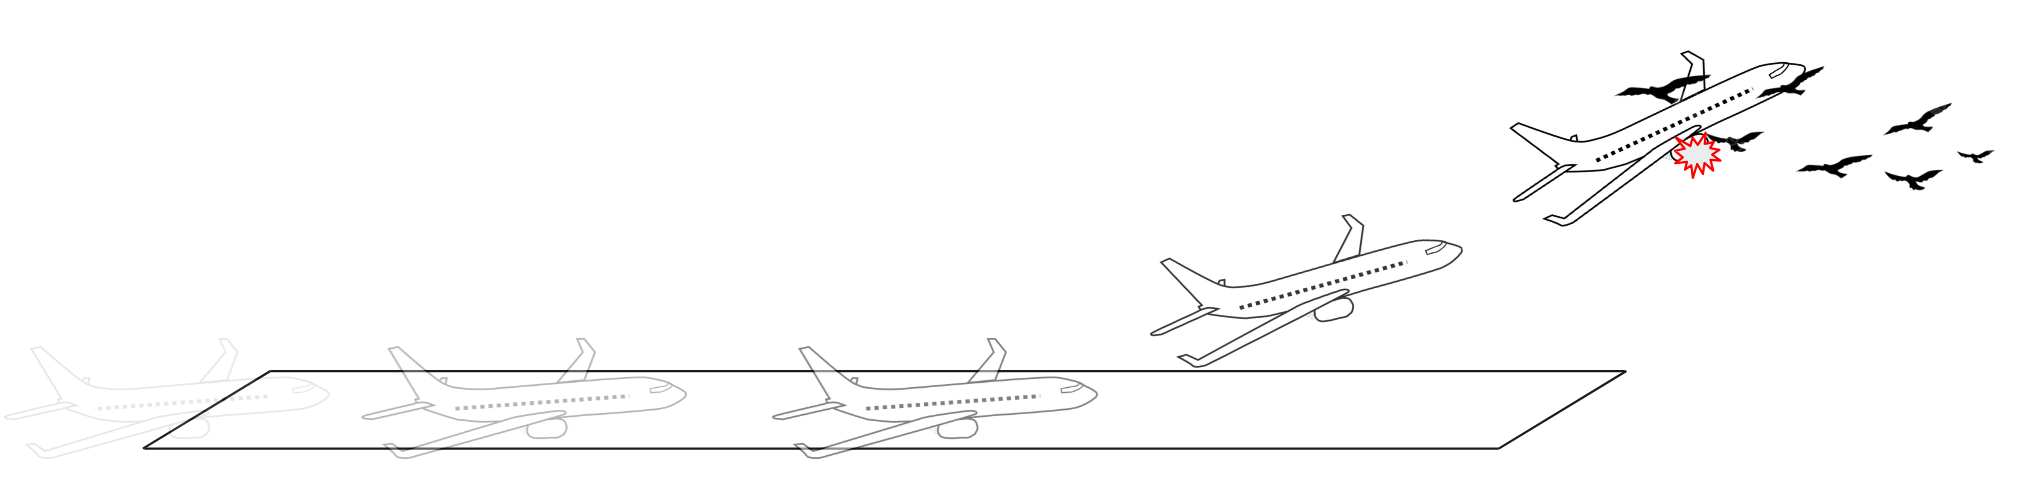
\includegraphics[width=1\textwidth]{./images/scenario.png}
   		\caption{Takeoff scenario with a birdstrike causing an engine failure.}
		\label{fig:your-image-label}
	\end{figure}


	\subsection{Phase 1: Work and design domain analysis}
	The first step of the methodology involves analyzing the current state of commercial aviation operations to understand the design domain of the to-be-designed Autonomous Agent (AA). Two complementary methods are used, the Goal Directed Task Analysis (GDTA) and the Interdependence Analysis (IA).

	\subsubsection{Goal-Directed Task Analysis}
	A GDTA was conducted to understand the information needs inherent to commercial aviation operations. GDTA is a task analysis methodology aimed at identifying the critical information human operators must acquire and process to achieve their mission goals effectively and safely. This information contributes to the construction and maintenance of Situation Awareness (SA), a key predictor of operational performance and safety in commercial aviation \parencite{endsley_here_2017}. %Verify this ref, goal is to say SA is predictor of operational performance. SotA on SA might be good
	Following the established GDTA outlined by Endsley and Jones for a complete commercial aviation flight \parencite{endsley_designing_2003}, our GDTA was constructed by selecting the relevant hierarchy of goals and associated information requirements for our takeoff scenario. To enrich and validate the GDTA, four experienced commercial pilots were recruited and interviewed. Their insights were incorporated to ensure that the analysis reflects the operational realities of contemporary flight environments.

	The GDTA resulted in a hierarchically organized representation of pilot goals, each associated with the specific information necessary for optimal task performance. This structured output serves as a foundation for designing the human-autonomy team. Specifically, the identified information elements will guide the development of the Autonomous Agent, ensuring that both the human pilot and the synthetic teammate maintain a sufficient level of SA throughout the operation.

	The goal is to ensure that the closely coupled human-agent team maintains alignment of their respective situation representation by attending both to the proper information for the task at hand. This alignment supports the development of Team Situation Awareness (Team SA)—the state in which each teammate possesses an accurate understanding of the situation relevant to their roles within the flight deck.
	This notion is visually represented by Figure~\ref{fig:team-sa-venn}, where individual SA of each team member contributes to the larger construct of Team SA. Furthermore, a significant overlap in individual SA defines the concept of Shared Situation Awareness. Achieving and maintaining both individual SA and shared SA between the human and autonomous teammate is critical to ensuring coordinated, safe, and effective operations.

	\begin{figure}[h!]
		\centering
		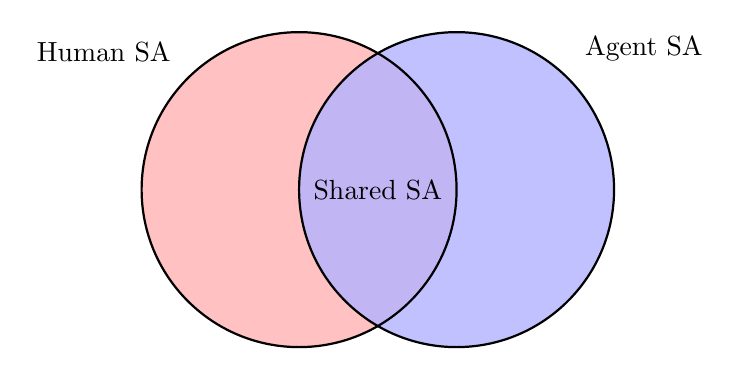
\begin{tikzpicture}
        % Left circle (Human SA)
        \fill[red!30, opacity=0.8] (-1,0) circle (2);
        % Right circle (Agent SA)
        \fill[blue!30, opacity=0.8] (1,0) circle (2);

        % Borders
        \draw[thick] (-1,0) circle (2) node[above left=1.5cm] {Human SA};
        \draw[thick] (1,0) circle (2) node[above right=1.5cm] {Agent SA};

        % Label overlap
        \node at (0,0) {Shared SA};
		\end{tikzpicture}
		\caption{Venn diagram illustrating Team Situation Awareness (Team SA) with the overlapping individual SA of the human pilot and the autonomous agent representing Shared SA.}
		\label{fig:team-sa-venn}
	\end{figure}

	\subsubsection{Interdependence Analysis}
	Interdependent Analysis is a work analysis methods part of the coactive design process that helps improve collaboration between humans and machines by identifying key interdependence relationships that are essential for effective teamwork \parencite{johnson_coactive_2014}. It also defines the requirements for tasks that involve interdependence, ensuring successful cooperation. This framework consists of three main parts: (1) joint activity modeling, (2) interdependence assessment, and (3) workflow analysis. These components help guide the design of systems for more effective teamwork, particularly in human-autonomy teams \parencite{johnson_understanding_2018}.
	To define human and autonomy role for our case study we have performed an Interdependence Analysis. This tool's most powerful feature is its ability to map different teaming options at the beginning of the design process, as opposed to a single function allocation solution. The output of an IA gives:
	\begin{itemize}
		\item Different teaming alternatives, especially in our case the dyad human-agent with human as main performer of the activity and agent as supporter or conversely agent as the main performer and human as the supporter.
		\item A visualization of possible workflows for the team to carry-out the activity, depending on the team alternative, required, and opportunistic interdependence relationship.
		\item A list of \textbf{Observability, Predictability, and Directability} requirements to ensure proper collaboration for the human-autonomy team.
	\end{itemize}
	\subsection{Phase 2: Cognitive modeling and agent development}

	\begin{figure}[h!]
		\centering
		% First logo
		\begin{minipage}[b]{0.3\textwidth}
			\centering
			\raisebox{2mm}{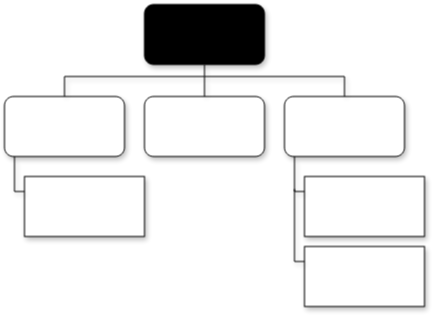
\includegraphics[width=0.9\textwidth]{images/hierarchy_diagram.png}}
		\end{minipage}
		% Second logo
		\begin{minipage}[b]{0.3\textwidth}
			\centering
			
\includegraphics[width=0.6\textwidth]{images/workflow_icon.png}
		\end{minipage}
		% Third logo
		\begin{minipage}[b]{0.3\textwidth}
			\centering
			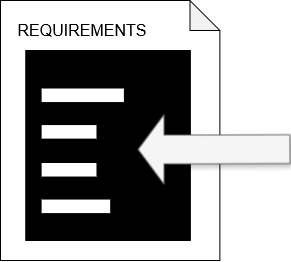
\includegraphics[width=0.8\textwidth]{images/requirements.png}
		\end{minipage}
		\caption{Output of phase 1 - goal hierarchy, task workflow, information \& OPD requirements.}
		\label{fig:logos}
	\end{figure}

	\subsubsection{QN-ACTR}
	\subsubsection{SEEV}
	\subsubsection{Agent design}
	\subsubsection{System architecture}
	\subsubsection{Scenario \& Simulation}
	\subsection{Phase 3: Human-In-The-loop simulation studies}
	\subsubsection{Scenario}
	\subsubsection{Equipment}
	\subsubsection{Participants}
	\subsubsection{Protocol}
	\subsubsection{Model validation and results}
	
	\section{Expected Results} % Section for expected results
	\begin{itemize}
		\item A cognitive model predicting pilot cognitive load and situation awareness.
		\item An evaluation of human-autonomy cooperation strategies.
		\item Empirical validation via HITLS to assess acceptance of the autonomous co-pilot.
	\end{itemize} % Lists expected outcomes
	
	\section{Originality and Impact} % Section for originality and impact
	This project provides an advanced methodology for integrating collaborative autonomous systems into the cockpit, improving the safety and efficiency of Single Pilot Operations.
	
	\section{Risks assessment and mitigation}
	My risks
	
	\section{Resource management}
	My resources
	
	\section{Timeline}
	\printbibliography % Prints the bibliography
	
\end{document} % Ends the document
